\documentclass[a4paper, oneside]{report}
\usepackage[italian]{babel}
\usepackage[utf8]{inputenc}
\usepackage[a4paper,top=2.5cm,bottom=2.5cm,left=2cm,right=2cm]{geometry}
\usepackage[table,xcdraw]{xcolor}
\usepackage{booktabs}
\usepackage{pdfpages}
\usepackage{pgfplots}
\usepackage{fancyhdr}
\usepackage{caption}
\usepackage{subcaption}
\usepackage{hyperref}
\usepackage{amsmath}
\usepackage{amssymb}
\usepackage{soul}

\usepackage{algorithm}
\usepackage{algpseudocode}

\pagestyle{fancy}
\fancyhead[L,RO]{\slshape \rightmark}
\fancyfoot[C]{\thepage}

\title{Progetto Calcolo scientifico}
\author{
    Telemaco Terzi (\href{https://github.com/Tezze2001}{@Tezze2001}) \\\\
    Tommaso Ferrario (\href{https://github.com/TommasoFerrario18}{@TommasoFerrario18})
    }
\date{\today}

\pgfplotsset{compat=1.13}

\begin{document}

\maketitle
\newtheorem{teorema}{Teorema}
\newtheorem{dimostrazione}{Dimostrazione}
\newtheorem{definizione}{Definizione}
\newtheorem{esempio}{Esempio}

\tableofcontents

\chapter{Progetto 1 bis: Mini libreria per sistemi lineari}
\section{Introduzione}
Per la realizzazione della libreria contenente i metodi per la risoluzione di
sistemi lineari, è stato scelto di utilizzare \href{https://julialang.org/}{\textbf{Julia}},
un linguaggio di programmazione open-source, sviluppato per ottenere prestazioni
elevate e con una sintassi simile a quella di Python e MATLAB. Essendo concepito
per la manipolazione efficace del calcolo scientifico, offre una vasta gamma di
librerie per la gestione di matrici e vettori.

In particolare, per lo sviluppo di questo progetto sono state utilizzate due
librerie della Standard Library di Julia:
\begin{itemize}
    \item \textbf{LinearAlgebra}: fornisce funzioni per la manipolazione di
          matrici e vettori.
    \item \textbf{SparseArrays}: fornisce funzioni per la gestione di matrici sparse.
\end{itemize}

L'impiego di quest'ultima libreria è stato fondamentale per ridurre l'occupazione
di memoria, in quanto le matrici utilizzate negli esperimenti sono matrici sparse.
Nello specifico, sono state utilizzate le seguenti matrici sparse:
\begin{itemize}
    \item \textbf{spa1}: matrice di dimensione 1000x1000 con 182,434 elementi non nulli.
    \item \textbf{spa2}: matrice di dimensione 3000x3000 con 1,633,298 elementi non nulli.
    \item \textbf{vem1}: matrice di dimensione 1681x1681 con 13,385 elementi non nulli.
    \item \textbf{vem2}: matrice di dimensione 2601x2601 con 21,225 elementi non nulli.
\end{itemize}

Per permettere la riproducibilità degli esperimenti, vogliamo riportare di seguito
le caratteristiche del sistema utilizzato per la realizzazione della libreria e
per l'esecuzione degli esperimenti. Tutti gli esperimenti sono stati eseguiti su
un computer con le seguenti caratteristiche:
\begin{itemize}
    \item CPU: Intel Core i5-1135G7
    \item RAM: 16 GB
    \item Sistema Operativo: Windows 11
    \item Julia: versione 1.10.2
\end{itemize}
\section{Struttura della libreria}
La libreria realizzata è composta da tre moduli principali:
\begin{itemize}
    \item \textbf{IterativeMethods}: contiene i metodi iterativi per la risoluzione
          di sistemi lineari.
    \item \textbf{DirectMethods}: contiene i metodi diretti per la risoluzione
          di sistemi lineari.
    \item \textbf{Utils}: contiene le funzioni di utilità per la manipolazione
          di matrici e vettori.
\end{itemize}

\subsection{Utils}
Nel modulo \textbf{Utils} sono presenti le funzioni per svolgere compiti di
utilità. Tra queste troviamo:
\begin{itemize}
    \item \textbf{read\_sparse\_matrix}: funzione per la lettura di una matrice
          da file in formato \textbf{.mtx}. Tale funzione restituisce una matrice
          sparsa.
    \item \textbf{check\_sizes}: funzione per il controllo delle dimensioni di
          una matrice e del vettore dei termini noti.
\end{itemize}
\subsection{DirectMethods}
Nel modulo \textbf{DirectMethods} è presente il metodo che effettua la risoluzione
di un sistema lineare in cui la matrice è triangolare inferiore, tramite il
metodo di sostituzione in avanti.

Di seguito riportiamo lo pseudocodice del metodo \textbf{forward\_substitution}:
\begin{verbatim}
function forward_substitution(A, b)
    n = size(A, 1)
    x = zeros(n)
    x[1] = b[1] / A[1, 1]
    for i in 2
        x[i] = (b[i] - dot(A[i, 1], x[1])) / A[i, i]
    end
    return x
end
\end{verbatim}
Questo metodo è stato implementato poiché nel metodo di risoluzione di Gauß-Seidel,
per cui la regola di aggiornamento è la seguente:
\begin{equation}
    x^{(k+1)} = x^{(k)} + P^{-1}(b - Ax^{(k)})
\end{equation}
con $P$ è una matrice triangolare inferiore, prevede il calcolo di una matrice
inversa. Dato che tale operazione è computazionalmente costosa, possiamo evitare
di calcolare la matrice inversa e al suo posto risolvere il seguente sistema
lineare:
\begin{equation}
    Py = b - Ax^{(k)}
\end{equation}
dove $y$ è il vettore che otteniamo risolvendo il sistema lineare con il metodo
della sostituzione in avanti. In questo modo, possiamo calcolare la soluzione
$x^{(k+1)}$ come:
\begin{equation}
    x^{(k+1)} = x^{(k)} + y
\end{equation}
\subsection{IterativeMethods}
Nel modulo \textbf{IterativeMethods} sono presenti i metodi iterativi per la
risoluzione di sistemi lineari. In particolare, sono stati implementati i seguenti
metodi:
\begin{itemize}
    \item \textbf{Jacobi}: metodo di Jacobi per la risoluzione di sistemi lineari.
    \item \textbf{GaussSeidel}: metodo di Gauß-Seidel per la risoluzione di
          sistemi lineari.
    \item \textbf{Gradient}: metodo del gradiente per la risoluzione di sistemi
          lineari.
    \item \textbf{ConjugateGradient}: metodo del gradiente coniugato per la
          risoluzione di sistemi lineari.
\end{itemize}

Tutti i metodi implementati utilizzano come criterio di arresto il confronto del
residuo riscalato, calcolato come:
\begin{equation}
    \frac{\|b - Ax^{(k)}\|}{\|b\|}
\end{equation}
dove $x^{(k)}$ è la soluzione al passo $k$ e $b$ è il vettore dei termini noti.
La tolleranza per questo confronto è un valore fornito dall'utente.

Inoltre, per evitare cicli infiniti, è possibile specificare un numero massimo
di iterazioni. Il valore predefinito è fissato a 20000 iterazioni.

La libreria è stata progettata a partire dalla definizione di una funzione generica
\textbf{GenericIterativeMethod}, la quale prende in input la matrice $A$, il
vettore dei termini noti $b$, la tolleranza, il numero massimo di iterazioni, e
il metodo di aggiornamento della soluzione. Questa funzione implementa una logica
comune a tutti i metodi iterativi, come rappresentato dal seguente pseudocodice:
\begin{verbatim}
function GenericIterativeMethod(A, b, tol, max_iter, update_method)
    n = size(A, 1)
    x = zeros(n)
    r = b - A * x
    res = norm(r) / norm(b)
    iter = 0
    while res > tol
        x = update_method(A, b, x)
        r = b - A * x
        res = norm(r) / norm(b)
        iter += 1
        if iter == max_iter
            print("Numero massimo di iterazioni raggiunto")
            return x
        end
    end
    return x
end
\end{verbatim}

Per ciascun metodo iterativo richiesto, è stato definito un metodo specifico che
implementa la regola di aggiornamento della soluzione. Questo metodo restituisce
la soluzione aggiornata al passo $k+1$ e, dato che il criterio di arresto è basato
sul residuo riscalato, tutti i metodi richiedono il calcolo del residuo. Pertanto,
è stato deciso di restituire anche il residuo calcolato, per evitare di ricalcolarlo
ogni volta. La logica di aggiornamento della soluzione sfrutta le funzioni per
la manipolazione di matrici e vettori fornite dalla libreria \textbf{LinearAlgebra}.

In aggiunta, la libreria contiene metodi di interfaccia che richiamano direttamente
la funzione generica, passando il metodo di aggiornamento corrispondente al metodo
iterativo richiesto.

Di seguito sono presentate le implementazioni dei metodi iterativi richiesti.

\subsubsection{Metodo di Jacobi}
Per il metodo di Jacobi, la regola di aggiornamento della soluzione è la seguente:
\begin{equation}
    x^{(k+1)} = x^{(k)} + P^{-1}(b - Ax^{(k)})
\end{equation}
In questo caso, il calcolo della matrice inversa $P^{-1}$ è efficiente poiché $P$
è una matrice diagonale; di conseguenza, basta calcolare il reciproco degli
elementi sulla diagonale.

Durante la definizione di questo metodo, è stata prevista l'implementazione dei
metodi \textbf{JOR} e \textbf{Richardson}, introducendo i parametri $\omega$ e
$\alpha$, con i relativi controlli per verificarne la presenza e gli intervalli
di valori ammissibili.

\subsubsection{Metodo di Gauß-Seidel}
Per il metodo di Gauß-Seidel, la regola di aggiornamento della soluzione è la seguente:
\begin{equation}
    x^{(k+1)} = x^{(k)} + y
\end{equation}
dove $y$ è il vettore ottenuto risolvendo il sistema lineare $Py = b - Ax^{(k)}$.
Questo è possibile poiché la matrice $P$ è una matrice triangolare inferiore,
quindi possiamo utilizzare il metodo della sostituzione in avanti per risolvere
il sistema lineare, evitando il calcolo della matrice inversa.

Anche per questo metodo è stata prevista l'implementazione dei metodi \textbf{SOR}
e \textbf{Richardson}, introducendo i parametri $\omega$ e $\alpha$, con i relativi
controlli per verificarne la presenza e gli intervalli di valori ammissibili.

\subsubsection{Metodo del Gradiente}
Per il metodo del gradiente, la regola di aggiornamento della soluzione è la seguente:
\begin{equation}
    x^{(k+1)} = x^{(k)} + \alpha r^{(k)}
\end{equation}
dove $r^{(k)}$ è il residuo al passo $k$ e $\alpha$ è il fattore di scala calcolato
come:
\begin{equation}
    \alpha = \frac{\langle r^{(k)}, r^{(k)}\rangle}{\langle r^{(k)}, Ar^{(k)}\rangle}
\end{equation}

\subsubsection{Metodo del Gradiente Coniugato}
Questo metodo rappresenta una versione migliorata del metodo del gradiente, in
cui si evita il problema della convergenza a "zig-zag". La regola di aggiornamento
della soluzione è la seguente:
\begin{equation}
    x^{(k+1)} = x^{(k)} + \alpha d^{(k)}
\end{equation}
dove $\alpha$ è il fattore di scala calcolato come:
\begin{equation}
    \alpha = \frac{\langle d^{(k)}, r^{(k)}\rangle}{\langle d^{(k)}, Ad^{(k)}\rangle}
\end{equation}
e $d^{(k)}$ è la direzione di discesa al passo $k$, calcolata ad ogni iterazione
con la formula:
\begin{equation}
    d^{(k)} = r^{(k)} + \beta_{k-1} d^{(k-1)}
\end{equation}
dove $\beta$ è il fattore di scala calcolato come:
\begin{equation}
    \beta_k = \frac{\langle d^{(k)T}, (Ar^{(k + 1)})\rangle}{\langle d^{(k)T}, (Ad^{(k)})\rangle}
\end{equation}
con $\langle \cdot, \cdot \rangle$ è il prodotto scalare tra due vettori.

\section{Risultati sperimentali}
Implementati i metodi, si è proceduto con la valutazione delle prestazioni di
ciascuno di essi. In particolare, sono stati eseguiti degli esperimenti sulle
matrici precedentemente descritte, utilizzando come vettore dei termini noti il
risultato della moltiplicazione tra la matrice e un vettore di 1 di dimensione
pari al numero di righe della matrice. Oltre a questo, i metodi sono stati testati
al variare della tolleranza, utilizzando i valori $1e^{-5}$, $1e^{-7}$, $1e^{-9}$
e $1e^{-11}$.

Per quanto riguarda le misurazioni dei tempi di esecuzione e l'occupazione di
memoria, sono state utilizzate la funzione \textbf{time}, invocata prima e dopo
l'esecuzione del codice, e la macro \textbf{@allocated} per misurare l'occupazione
di memoria. Quest'ultima restituisce la quantità di memoria allocata in byte.

Ogni metodo è stato eseguito 10 volte per ciascuna matrice e livello di tolleranza,
al fine di valutare la consistenza dei risultati. Una volta ottenuti i dati, si è
proceduto con la loro visualizzazione mediante grafici. In particolare, sono stati
realizzati grafici che mostrano i tempi di esecuzione e l'occupazione di memoria
in funzione della tolleranza per ciascuna matrice, consentendo un confronto tra
i diversi metodi.

Nei grafici l'andamento dei metodi è stato rappresentato attraverso la media delle
esecuzione e un'ombra che rappresenta la deviazione standard delle misurazioni.

Iniziamo analizzando i risultati ottenuti per il tempo di esecuzione dei metodi
sono riportati nelle figure \ref{fig:time_spa1}, \ref{fig:time_spa2}, \ref{fig:time_vem1}
e \ref{fig:time_vem2}.
% \begin{figure}[!ht]
%     \centering
%     \begin{subfigure}{0.45\textwidth}
%         \centering
%         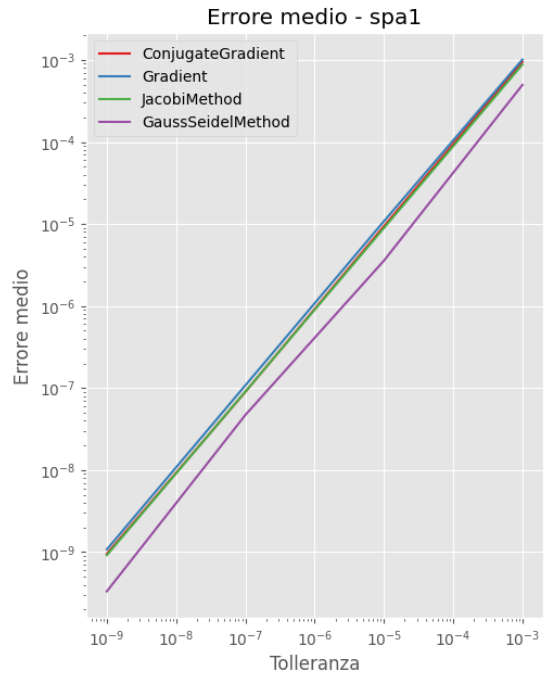
\includegraphics[width=\textwidth]{./img/error_spa1.png}
%         \caption{Matrice spa1}
%         \label{fig:time_spa1}
%     \end{subfigure}
%     \hfill
%     \begin{subfigure}{0.45\textwidth}
%         \centering
%         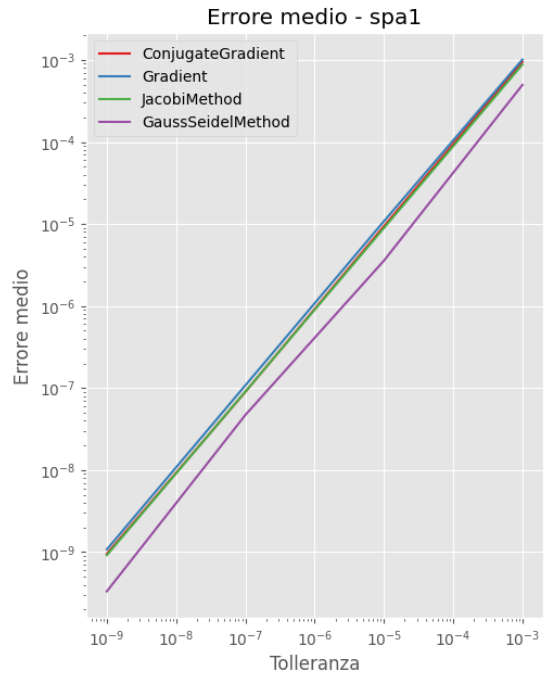
\includegraphics[width=\textwidth]{./img/error_spa1.png}
%         \caption{Matrice spa2}
%         \label{fig:time_spa2}
%     \end{subfigure}
%     \hfill
%     \begin{subfigure}{0.45\textwidth}
%         \centering
%         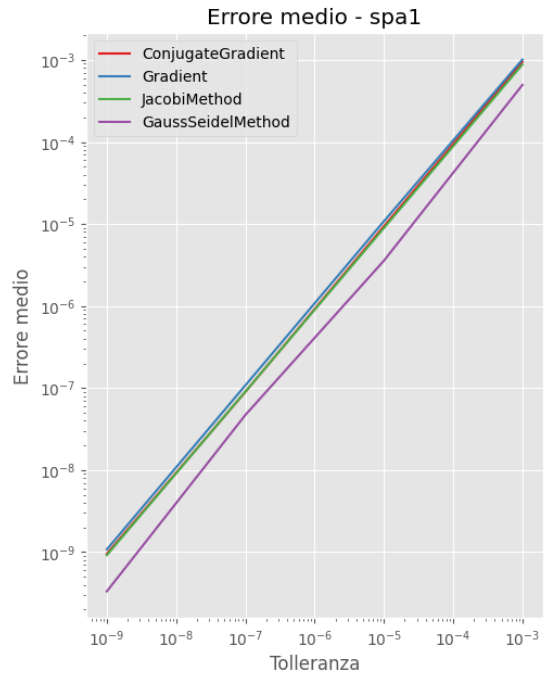
\includegraphics[width=\textwidth]{./img/error_spa1.png}
%         \caption{Matrice vem1}
%         \label{fig:time_vem1}
%     \end{subfigure}
%     \hfill
%     \begin{subfigure}{0.45\textwidth}
%         \centering
%         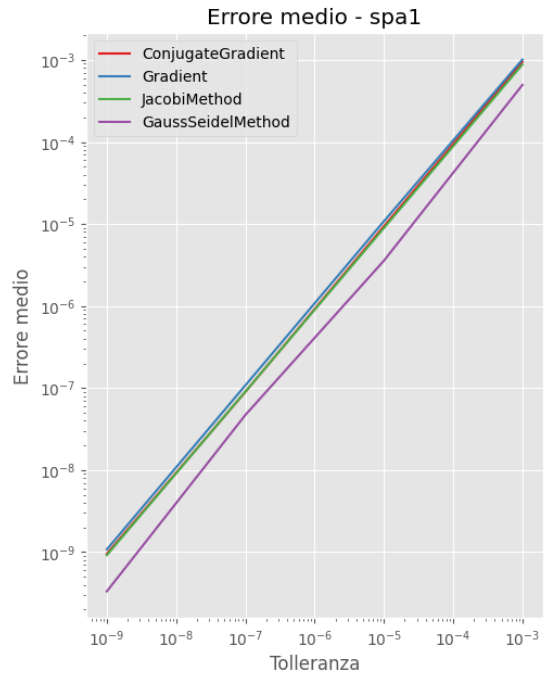
\includegraphics[width=\textwidth]{./img/error_spa1.png}
%         \caption{Matrice vem2}
%         \label{fig:time_vem2}
%     \end{subfigure}
%     \caption{Tempi di esecuzione dei metodi iterativi}
%     \label{fig:time}
% \end{figure}

In questi grafici, possiamo notare che il metodo di Gauß-Seidel risulta essere
il più lento per le matrici vem1 e vem2, mentre per le matrici spa1 e spa2
il metodo che richiede più tempo è il metodo del gradiente.

Per quanto riguarda l'occupazione di memoria, i risultati ottenuti sono riportati
nelle figure \ref{fig:mem_spa1}, \ref{fig:mem_spa2}, \ref{fig:mem_vem1} e \ref{fig:mem_vem2}.

% \begin{figure}[!ht]
%     \centering
%     \begin{subfigure}{0.45\textwidth}
%         \centering
%         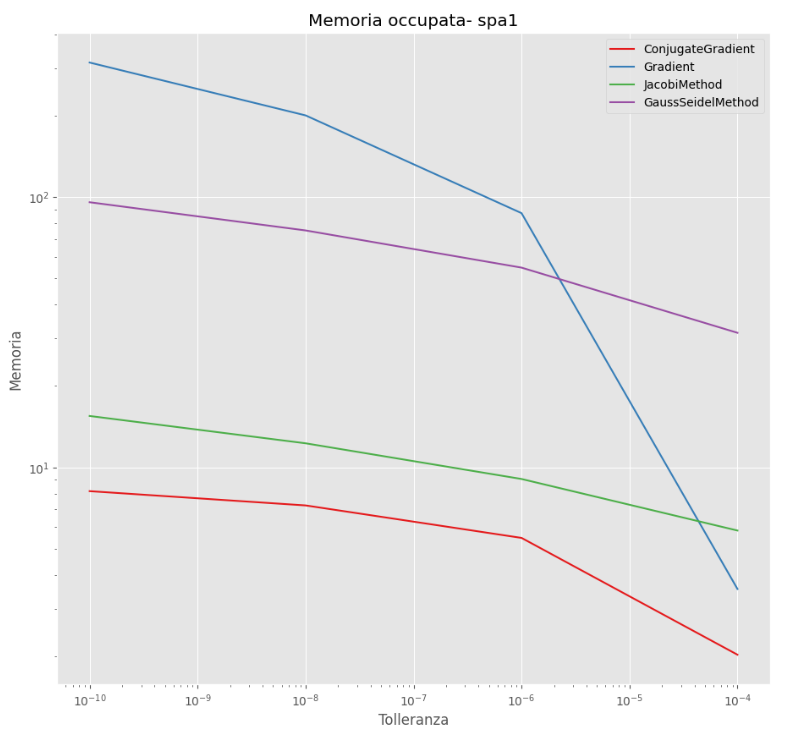
\includegraphics[width=\textwidth]{./img/mem_spa1.png}
%         \caption{Matrice spa1}
%         \label{fig:mem_spa1}
%     \end{subfigure}
%     \begin{subfigure}{0.45\textwidth}
%         \centering
%         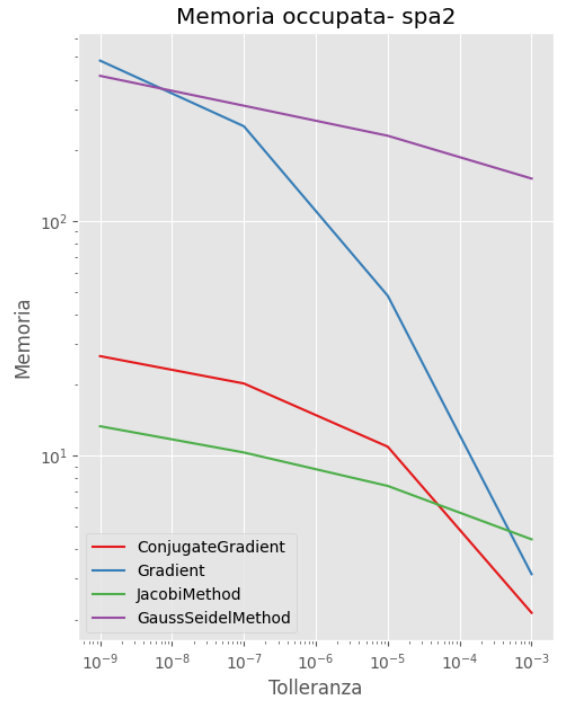
\includegraphics[width=\textwidth]{./img/mem_spa2.png}
%         \caption{Matrice spa2}
%         \label{fig:mem_spa2}
%     \end{subfigure}
%     \begin{subfigure}{0.45\textwidth}
%         \centering
%         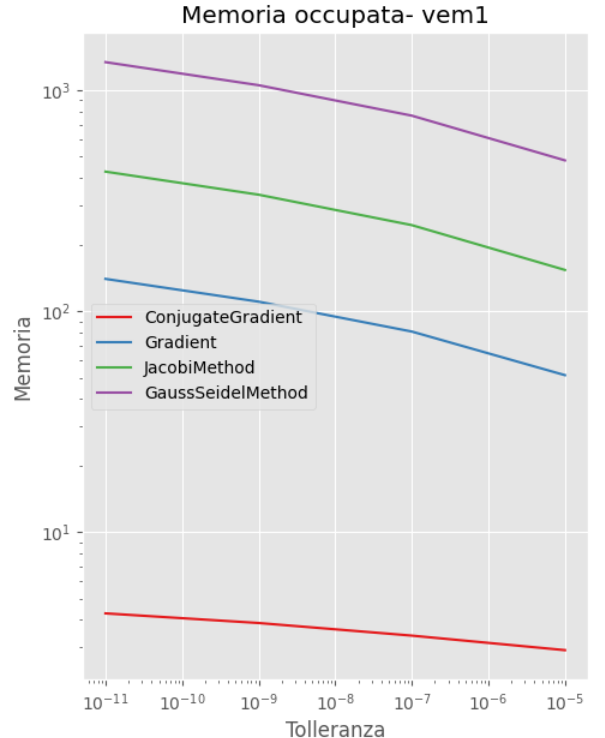
\includegraphics[width=\textwidth]{./img/mem_vem1.png}
%         \caption{Matrice vem1}
%         \label{fig:mem_vem1}
%     \end{subfigure}
%     \begin{subfigure}{0.45\textwidth}
%         \centering
%         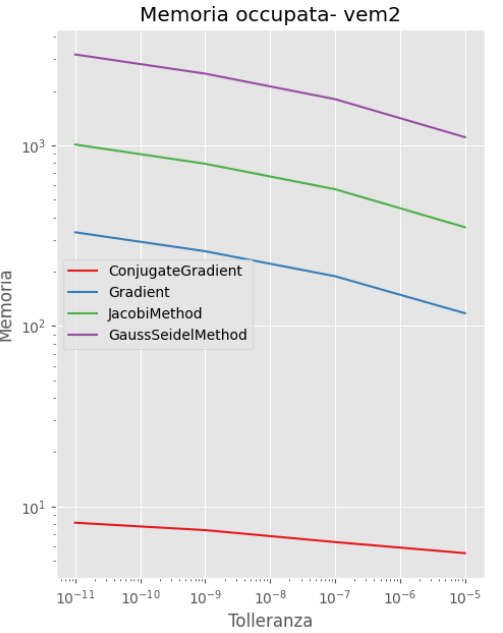
\includegraphics[width=\textwidth]{./img/mem_vem2.png}
%         \caption{Matrice vem2}
%         \label{fig:mem_vem2}
%     \end{subfigure}
%     \caption{Memoria occupata dei metodi iterativi}
%     \label{fig:memory}
% \end{figure}

In questi grafici, possiamo notare che il metodo di Gauß-Seidel risulta essere....


Infine, presentiamo i grafici che illustrano la variazione dell'errore medio in
funzione della tolleranza per ciascuna matrice, come mostrato nelle figure \ref{fig:error_spa1},
\ref{fig:error_spa2}, \ref{fig:error_vem1} e \ref{fig:error_vem2}.

% \begin{figure}[!ht]
%     \centering
%     \begin{subfigure}{0.45\textwidth}
%         \centering
%         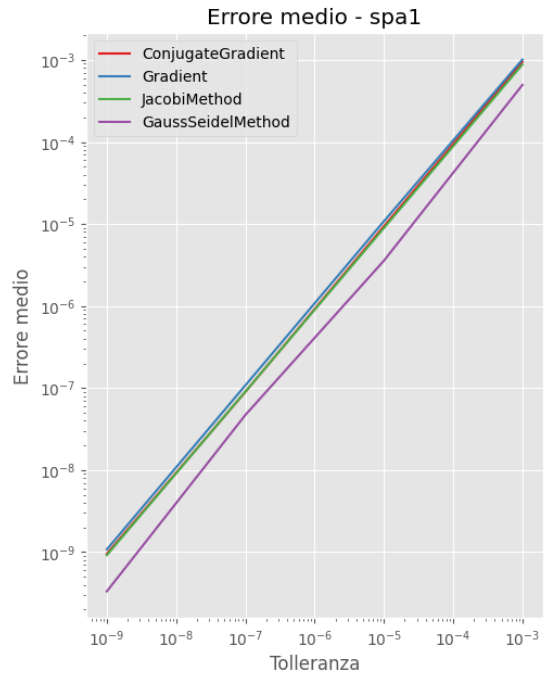
\includegraphics[width=\textwidth]{./img/error_spa1.png}
%         \caption{Matrice spa1}
%         \label{fig:error_spa1}
%     \end{subfigure}
%     \begin{subfigure}{0.45\textwidth}
%         \centering
%         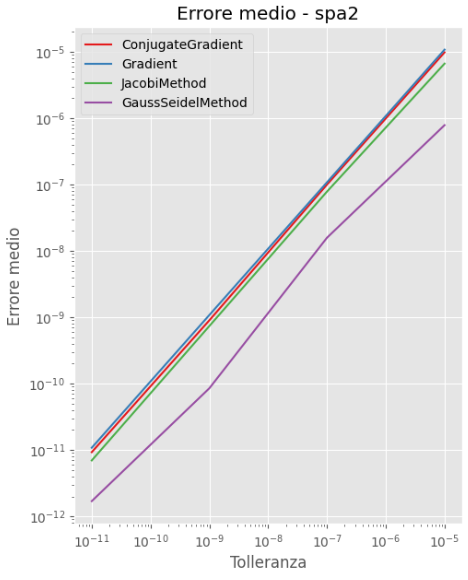
\includegraphics[width=\textwidth]{./img/error_spa2.png}
%         \caption{Matrice spa2}
%         \label{fig:error_spa2}
%     \end{subfigure}
%     \begin{subfigure}{0.45\textwidth}
%         \centering
%         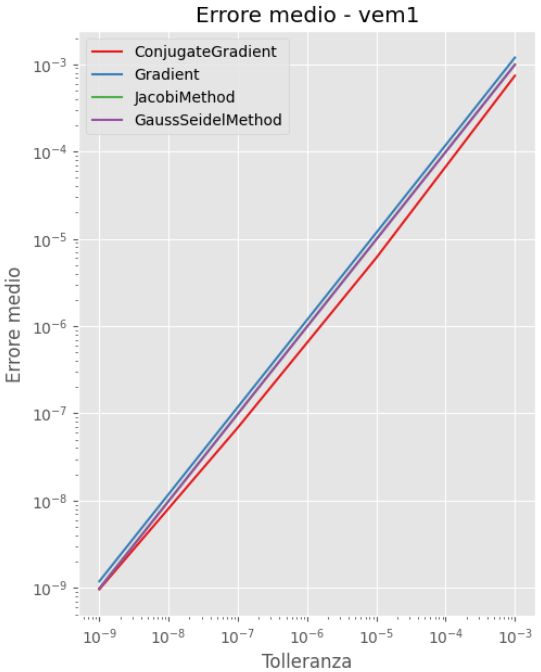
\includegraphics[width=\textwidth]{./img/error_vem1.png}
%         \caption{Matrice vem1}
%         \label{fig:error_vem1}
%     \end{subfigure}
%     \begin{subfigure}{0.45\textwidth}
%         \centering
%         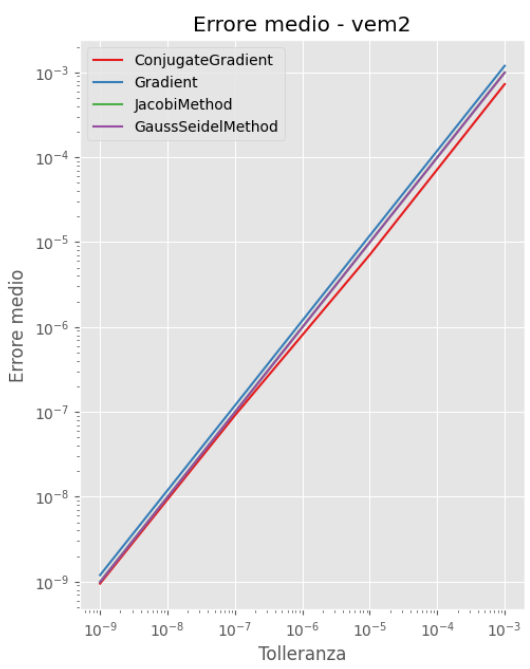
\includegraphics[width=\textwidth]{./img/error_vem2.png}
%         \caption{Matrice vem2}
%         \label{fig:error_vem2}
%     \end{subfigure}
%     \caption{Errore dei metodi iterativi}
%     \label{fig:error}
% \end{figure}

In questi grafici possiamo osservare un andamento che decresce più la tolleranza
si avvicina a zero. Questo è legato al fatto che tutti i metodi implementati
convergono prima di raggiungere il numero di iterazioni massimo (20000). Inoltre,
non si riesce a notare una differenza significativa tra i metodi implementati.

\chapter{Progetto 2: Compressione di immagini tramite la DCT}

\section{Introduzione}
In questo progetto è stata implementata l'equazione della discrete cosine transform $2$ (DCT2).
La sua implementazione è stata realizzata applicando sequenzialmente sulla matrice
la discrete cosine transform $1$ (DCT) per righe e poi per colonne. In questo modo
è stato possibile riutilizzare più efficacemente il codice senza introdurre code
smells.

L'intero progetto è stato sviluppato in Julia, un linguaggio di programmazione ad
alto livello usato per il calcolo scientifico con tempi di esecuzione comparabili
con C/C++.

La libreria della FFT di Julia utilizzata è \href{https://github.com/JuliaMath/FFTW.jl}{FTTW}
che implementa un binding con la libreria di C, entrambe le librerie sono open source.

\section{DCT2 custom}
Come preannunciato in precedenza, è stato necessario concentrarsi solo in una implementazione
efficiente della DCT, la sua formula è stata riportata nell'equazione \ref{eq:dct}.

\begin{equation}
    X_k = \begin{cases}
        \sqrt{\frac{1}{N}}\cdot \sum_{n=0}^{N-1} x_n \cos\left[\frac{\pi}{N}\left(n + \frac{1}{2}\right) n \right] & k=1     \\
        \sqrt{\frac{2}{N}}\cdot\sum _{n=0}^{N-1}x_{n}\cos \left[\frac{\pi}{N}\left(n+\frac{1}{2}\right)n\right]    & k \ne 1
    \end{cases}
    \label{eq:dct}
\end{equation}

Per prima cosa è stato pensato di utilizzare un approccio basato su operazioni
tra vettori e matrice, più precisamente è stato pensato di pre-calcolare la matrice
della base dei coseni, per righe, prima di effettuare il calcolo dei coefficienti.
Successivamente si effettua un prodotto vettore-matrice per ottenere il vettore
dei coefficienti, infine si applica la normalizzazione su di essi.

Dato un generico vettore $X_k$, per applicare la dct si effettua:
\begin{equation*}
    dct(X_k) = norm(B_{\cos}\cdot X_k )
\end{equation*}

Dove $\cdot$ è il prodotto vettore matrice e $B_{\cos}$ è la base dei coseni creata
per riga, mentre $X_k$ è il vettore colonna iniziale. La funzione di normalizzazione
normalizza i coefficienti del vettore risultante nel seguente modo, normalizza
per $\sqrt{\frac{1}{N}}$ il primo coefficiente, mentre gli altri li normalizza
per $\sqrt{\frac{2}{N}}$.

L'implementazione della DCT2 si articola nel seguente modo:
\begin{itemize}
    \item si genera la base dei coseni per riga
    \item si applica inplace la DCT1 per righe
    \item si applica inplace la DCT1 per colonne
\end{itemize}

In questo modo si riescono ad ottenere dei tempi comparabili alla DCT2 implementata
dalla libreria usando la FFT.

\subsection{Studio di complessità}
L'algoritmo custom che è stato sviluppato ha dei tempi di esecuzione comparabili
con la libreria.

La complessità della DCT2 custom è la seguente:
\begin{itemize}
    \item \textbf{generazione della base dei coseni}: la generazione richiede
          un numero costante di operazioni tra scalari e un calcolo del coseno per ogni
          entry della matrice. Questo richiede un totale $\mathcal{O}(N^2)$ per generare
          la matrice, quando $N\times N$ è la dimensione della matrice (dimensione dello
          spazio vettoriale per numero di coefficienti).
    \item \textbf{applicazione della DCT1 su un vettore}: l'applicazione della DCT1
          su un generico vettore richiede di effettuare un prodotto matrice-vettore e
          successivamente di normalizzare i coefficienti. Il prodotto matrice-vettore
          ha una complessità asintotica di $\mathcal{O}(N^2)$, dove $N$ è la dimensione
          del vettore. Mentre per normalizzare i coefficienti si richiede una scansione
          lineare del vettore che richiede $\mathcal{O}(N)$, dove $N$ è la dimensione
          del vettore. Quindi complessivamente si ha una complessità di $\mathcal{O}(N^2 + N) = \mathcal{O}(N^2)$.
    \item \textbf{applicazione della DCT2 sull'intera matrice}: l'applicazione della DCT2
          sull'intera matrice richiede di eseguire una DCT1 per ogni riga e poi per ogni
          colonna. All'atto pratico non si rigenera ogni volta la matrice dei coseni,
          bensì inizialmente la si pre-calcola ($\mathcal{O}(N^2)$), successivamente si
          esegue la DCT1 per righe che richiede $\mathcal{O}(N \cdot N^2)$ ($N$ righe
          per $N^2$ la moltiplicazione riga-matrice) e successivamente si applica la
          DCT1 per colonne che richiede $\mathcal{O}(N \cdot N^2)$ ($N$ colonne
          per $N^2$ la moltiplicazione riga-matrice). Complessivamente si ottiene
          un $\mathcal{O}(N^3)$ a livello asintotico.
\end{itemize}

L'implementazione custom della DCT2 è stata confronta anche con quella ottimizzata
dalla libreria usando la FFT e nell'immagine \ref{fig:analisi_complex} si
può vedere il confronto.

\begin{figure}[!h]
    \centering
    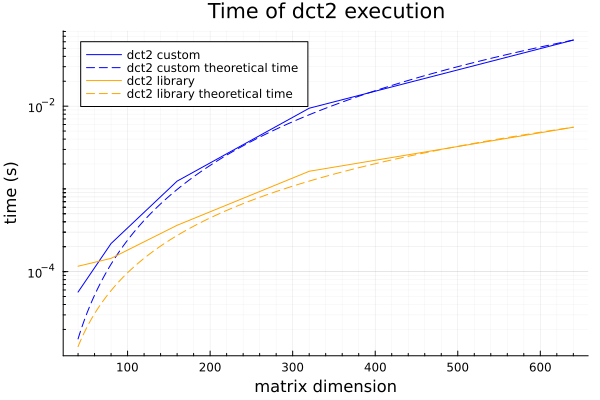
\includegraphics[width=0.5\textwidth]{Progetto_2/img/times_plot.png}
    \caption{Grafico dei tempi al variare della dimensione della matrice. Le linee
        continue rappresentano i dati empirici, le linee tratteggiate rappresentano
        l'andamento teorico dei metodi.}
    \label{fig:analisi_complex}
\end{figure}

Come si può notare dal grafico, l'andamento empirico segue quello teorico.

\section{Compressione}
In questa parte di progetto è stato implementata un'interfaccia web per ottenere
l'immagine bmp in scala di grigi

\subsection{Implementazione dell'interfaccia}

\subsection{Implementazione della compressione}
Dopo l'implementazione della GUI che si occupa di prendere in input l'immagine e
i due parametri, è stato sviluppato l'algoritmo di compressione dell'immagine.

L'implementazione della compressione si è articolata nel seguente modo:
\begin{itemize}
    \item \textbf{ridimensione dell'immagine in input}: l'immagine è stata ridimensionata
          in modo tale da avere altezza e larghezza multiple del parametro $f$.
    \item \textbf{implementazione della compressione}: la compressione è stata implementata
          applicando sui sotto-quadrati $f\times f$ dell'immagine la DCT2 della libreria,
          successivamente sono state azzerate le entry $k,l$ tali che $k+l\ge d$, infine
          si applica IDCT2 della libreria e si normalizzano i valori.
    \item \textbf{visualizzazione output}: infine vinee visualizzato l'output
          messo a confronto con l'input.
\end{itemize}

Nel dettaglio, la \textbf{ridimensione dell'immagine in input} elimina le ultime
righe e le ultime colonne dell'immagine in input in modo da avere le dimensioni
multiple di $f$.

Mentre, l'\textbf{implementazione della compressione} si articola nell'allocazione
di una matrice di appoggio $C\in \mathcal{R}^{f\times f}$ che viene inizializzata
su una sotto matrice $f\times f$ dell'immagine che si vuole elaborare.

\end{document}